\subsection{Interpretación del Modelo con SHAP}

Tras una exhaustiva investigación y comparación de algoritmos, se determinó que el modelo de clasificación más adecuado es el RandomForestClassifier. Dado que el objetivo principal de la investigación es determinar la aprobación del curso, este modelo se seleccionó para analizar la variable objetivo \say{aprobado}. Esta variable nos permite identificar si un estudiante aprobó o reprobó la primera evaluación y evaluar el impacto de la guía de apoyo en dicha aprobación. A continuación, se detallan los resultados y análisis de este modelo.

\subsubsection{Preparación y Selección de Características}

Para el análisis, se prepararon las coordenadas de análisis X/Y utilizando la columna \say{aprobado} como referencia para el eje Y. Esta columna es binaria, derivada de \say{sol1}, donde 1 indica aprobación con una nota mayor o igual a 4. El comportamiento de las demás columnas se analizará en relación con este eje.


\begin{lstlisting}[language=Python, caption=Selección de características y variable objetivo para RandomForestClassifier, label=lst:seleccion_caracteristicasRFC]
y = df["aprobado"]
X = df[
['hito1', 'hito2', 'exitosos', 'fallidos','e0', 'e1', 'e2', 'e3', 'e4', 'e5', 'e6', 'e7', 'e8', 'e9', 'e10', 'e11', 'e12', 'e13', 'e14', 'e15', 'e16', 'e17', 'e18', 'e19', 'e20', 'e21', 'e22', 'e23', 'e24', 'e25', 'e26', 'e27', 'e28', 'e29', 'e30', 'e31', 'e32', 'e33', 'e34', 'e35', 'e36', 'e37', 'e38', 'e39', 'e40', 'e41', 'e42', 'e43', 'e44', 'e45', 'e46', 'e47', 'e48', 'e49', 'e50', 'e51', 'e52']
]
\end{lstlisting}

\subsubsection{División de Datos y Definición del Modelo}

Para evaluar el rendimiento del modelo, se dividen los datos en conjuntos de entrenamiento (80\%) y prueba (20\%).

\begin{lstlisting}[language=Python, caption=División de datos para entrenamiento y prueba, label=lst:train_test_split_RFC]
X_train, X_test, y_train, y_test = train_test_split(X,y, test_size = 0.2,random_state= 1502)
\end{lstlisting}

El modelo RandomForestClassifier se define según la mejor configuración obtenida en la comparación de algoritmos.


\begin{lstlisting}[language=Python, caption=Definición del modelo RandomForestRegressor, label=lst:def_RFC]
model = RandomForestRegressor( 
    max_depth=10, 
    min_samples_split=10, 
    min_samples_leaf=5,
    random_state= 1502,
    n_estimators=500
)
\end{lstlisting}

\subsubsection{Validación Cruzada y Evaluación del Modelo}

Para obtener una evaluación robusta del modelo, se utiliza la técnica de Stratified K-Fold Cross-Validation.

\begin{lstlisting}[language=Python, caption=Realizar Stratified K-Fold Cross-Validation en los datos de entrenamiento, label=lst:skfold_train]
# Realizar Stratified K-Fold Cross-Validation en los datos de entrenamiento
from sklearn.model_selection import StratifiedKFold


kfold = StratifiedKFold(n_splits=10, shuffle=True, random_state=1502)

# Matrices para almacenar los resultados de validación cruzada
cv_scores = []
cv_predictions = []

for train_index, val_index in kfold.split(X_train, y_train):
    # Dividir los datos en conjuntos de entrenamiento y validación
    X_train_fold, X_val_fold = X_train.iloc[train_index], X_train.iloc[val_index]
    y_train_fold, y_val_fold = y_train.iloc[train_index], y_train.iloc[val_index]
    
    # Entrenar el modelo en el conjunto de entrenamiento del fold actual
    model.fit(X_train_fold, y_train_fold)

    # Realizar predicciones en el conjunto de validación del fold actual
    y_val_pred = model.predict(X_val_fold)

    # Calcular el error cuadrático medio en el conjunto de validación del fold actual
    fold_score = mean_squared_error(y_val_fold, y_val_pred)
    cv_scores.append(fold_score)

    # Almacenar las predicciones del fold actual para su uso posterior
    cv_predictions.extend(y_val_pred)

    # Calcular el coeficiente de determinación en el conjunto de validación del fold actual
    r2 = r2_score(y_val_fold, y_val_pred)
    print("Fold - Error cuadrático medio:", fold_score)
    print("Fold - Coeficiente de determinación (R2):", r2)
    print()

# Calcular la puntuación promedio de validación cruzada
avg_score = np.mean(cv_scores)
percentage_score = avg_score * 100
print("Promedio del error cuadrático medio en validación cruzada:", avg_score)
print("Promedio del error cuadrático medio en validación cruzada en %:", percentage_score)
\end{lstlisting}


Los resultados obtenidos en la validación cruzada proporcionan una visión clara del rendimiento del modelo en diferentes subconjuntos de datos. Estos resultados son esenciales para garantizar que el modelo no esté sobreajustado y pueda generalizar bien en datos no vistos.

A continuación, se presenta una tabla con los resultados de la validación cruzada Stratified K-Fold en los datos de entrenamiento:

\begin{table}[h]
    \centering
    \caption{Resultados Stratified K-Fold Cross-Validation en los datos de entrenamiento}
    \label{lst:res_skfold_train}
    \begin{tabular}{|c|c|c|}
        \hline
        \textbf{Fold} & \textbf{Error cuadrático medio} & \textbf{Coeficiente de determinación (R2)} \\
        \hline
        1             & 0.2234                          & 0.0994                                     \\
        2             & 0.2161                          & 0.1307                                     \\
        3             & 0.2400                          & 0.0295                                     \\
        ...           & ...                             & ...                                        \\
        \hline
        \multicolumn{3}{|c|}{Promedio del error cuadrático medio: 0.2174}                            \\
        \multicolumn{3}{|c|}{Promedio del error cuadrático medio en \%: 21.74}                       \\
        \hline
    \end{tabular}
\end{table}

Si el RMSE es 0, significa que el modelo predice perfectamente los valores reales. Cuanto más cerca esté el MSE o RMSE de cero, mejor será el rendimiento del modelo en términos de la diferencia entre las predicciones y los valores reales.


\subsubsection{Análisis SHAP}

El análisis SHAP (SHapley Additive exPlanations) es una técnica que permite interpretar las predicciones de modelos complejos. En este caso, se utiliza para entender cómo cada característica influye en las predicciones del modelo RandomForestClassifier.

\begin{lstlisting}[language=Python, caption=Predicción con SHAP utilizando el conjunto de prueba, label=lst:shap_analysis]
# Realizar la predicción con SHAP utilizando el conjunto de prueba (X_test)
explainer = shap.Explainer(model)
shap_values = explainer.shap_values(X_test)
\end{lstlisting}


Para comprender los gráficos SHAP y su relevancia en la interpretación de modelos de aprendizaje automático, es crucial familiarizarse con ciertos términos clave y conceptos fundamentales. Estos términos nos proporcionan una visión clara de cómo determinadas características afectan las predicciones del modelo:

\begin{itemize}
    \item \textbf{Higher}: Se refiere a instancias con valores más altos de una característica, que contribuyen positivamente a la predicción.

    \item \textbf{Lower}: Denota instancias con valores más bajos de una característica, que reducen el valor de la predicción.

    \item \textbf{Feature Value}: Corresponde al valor real de una característica para una instancia dada. En el contexto de los gráficos SHAP, nos ayuda a visualizar cómo se compara el valor de una característica con otros valores en el conjunto de datos.

    \item \textbf{Shap Value}: Es una métrica que muestra cuánto varía la predicción del modelo debido a la presencia de una característica en particular. Un valor SHAP positivo sugiere que la característica incrementa la predicción, mientras que un valor negativo sugiere lo contrario.
\end{itemize}

\subsubsection{Visualización de Resultados con Gráficos SHAP}

Los gráficos SHAP ofrecen una representación visual detallada de la influencia de cada característica en las predicciones del modelo. A continuación, se presentan gráficos que destacan la importancia y el impacto de las características en las predicciones.

La Figura \ref{fig:caract_var_shap} ilustra el gráfico de importancia de características basado en valores SHAP.

\begin{figure}[H]
    \centering
    \begin{minipage}{0.48\textwidth}
        \begin{lstlisting}[language=Python, caption=Grafico de Caracteristicas, label=lst:graf_caracteristicas]
# Mostrar Grafico de Caracteristicas
shap.summary_plot(shap_values, X_test)
        \end{lstlisting}
    \end{minipage}
    \hfill
    \begin{minipage}{0.48\textwidth}
        \centering
        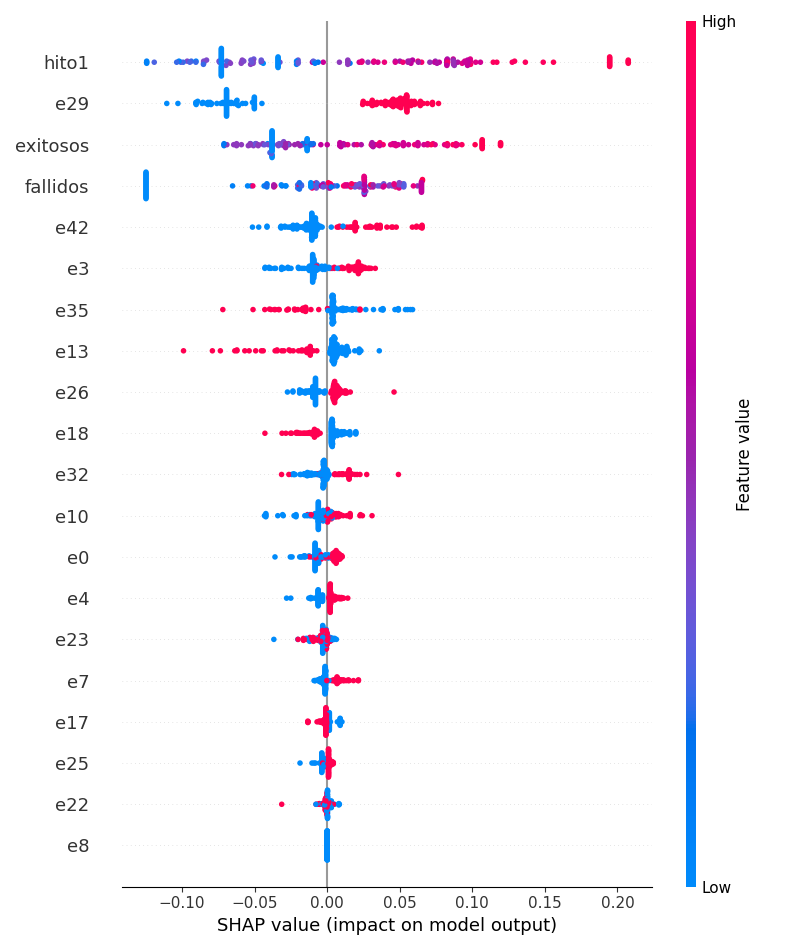
\includegraphics[width=0.9\linewidth]{img/shap_rf/shapForcePlot2.png}
        \caption{Importancia de Características basado en SHAP}
        \label{fig:caract_var_shap}
    \end{minipage}
\end{figure}

El gráfico SHAP, en particular el \textit{summary plot}, visualiza la importancia de cada característica y cómo afectan las predicciones. Cada punto en el gráfico representa un valor SHAP para una característica y una instancia específica. La posición en el eje Y del gráfico indica qué característica es y la posición en el eje X muestra si la presencia de esa característica aumenta o disminuye la predicción. Los colores representan el valor de la característica, siendo el azul para valores bajos y el rojo para valores altos. Las características se ordenan en función de su importancia, con las más importantes en la parte superior.

Esta visualización permite identificar rápidamente qué características son las más influyentes para el modelo y cómo la variación en los valores de estas características afecta las predicciones.

De la visualización, se observa que las características más influyentes son: \texttt{hito1}, \texttt{e29}, \texttt{exitosos}, \texttt{fallidos}, \texttt{e42}, \texttt{e3}, entre otras. Específicamente, \texttt{hito1} muestra una amplia gama de valores SHAP, extendiéndose tanto en tonos azules como rojos. La presencia de valores SHAP más anchos y separados indica la existencia de valores atípicos. Esto concuerda con lo observado en la tabla \ref{tab:valores_atipicos} presentada anteriormente, donde \texttt{hito1} tiene un valor destacado de 42.

Para visualizar la importancia numérica de cada característica de manera gráfica, se puede recurrir a la representación proporcionada por SHAP. Esta visualización facilita el análisis del impacto de cada característica en las predicciones del modelo:

\begin{figure}[H]
    \centering
    \begin{minipage}{0.48\textwidth}
        \begin{lstlisting}[language=Python, caption=Análisis de Importancia de Características, label=lst:cod_calvaloreshap]
# Análisis de Importancia de Características
shap_values_tree = explainer(X_test[:])
shap.plots.bar(shap_values_tree[0])
        \end{lstlisting}
    \end{minipage}
    \hfill
    \begin{minipage}{0.48\textwidth}
        \centering
        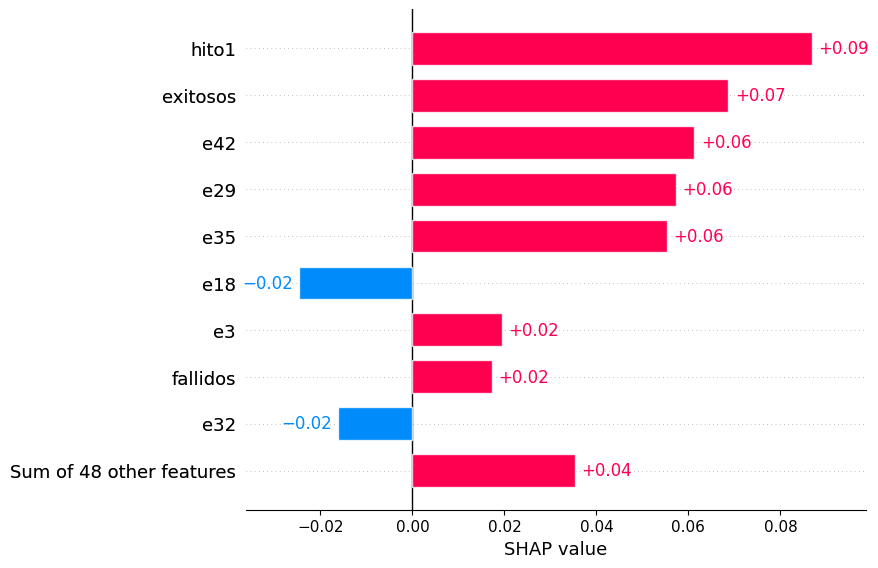
\includegraphics[width=0.9\linewidth]{img/shap_rf/ImportanciaDeCaracteristicasShap.png}
        \caption{Importancia de las Características según SHAP}
        \label{fig:importancia_relativa_shap}
    \end{minipage}
\end{figure}

La Figura \ref{fig:importancia_relativa_shap} ilustra la importancia relativa de las características según SHAP, poniendo de relieve las características con mayor influencia en las predicciones del modelo.

Para interpretar el gráfico \ref{fig:importancia_relativa_shap}, consideremos dos ejemplos:

\textbf{hito1 con +0.09 (color rojo y barra hacia la derecha)}:
\begin{itemize}
    \item \textbf{Dirección}: La barra orientada hacia la derecha sugiere que, en promedio, esta característica incrementa el valor de la predicción.
    \item \textbf{Color}: El tono rojo indica un impacto positivo en la predicción, lo que significa que valores más altos de \say{hito1} tienden a elevar la predicción.
    \item \textbf{Magnitud}: El valor +0.09 indica que, en promedio, un incremento en \say{hito1} eleva la predicción en 0.09 unidades (según la unidad de la variable objetivo).
\end{itemize}


\textbf{e18 con -0.02 (color azul y barra hacia la izquierda)}:
\begin{itemize}
    \item \textbf{Dirección}: La barra orientada hacia la izquierda sugiere que, en promedio, esta característica reduce el valor de la predicción.
    \item \textbf{Color}: El tono azul indica un impacto negativo en la predicción, lo que significa que valores más altos de \say{e18} tienden a reducir la predicción.
    \item \textbf{Magnitud}: El valor -0.02 señala que, en promedio, un incremento en \say{e18} reduce la predicción en 0.02 unidades.
\end{itemize}


Además, se presenta otro gráfico generado por matplotlib sobre la prediccion del modelo en la Figura \ref{fig:caract_var_shap_mat}:

\begin{lstlisting}[language=Python, caption=grafico matplotib, label=lst:graf_matplotib]
# Crear la figura de matplotlib
shap.force_plot(explainer.expected_value, shap_values[0,:], X_test.iloc[0,:], matplotlib=True)
\end{lstlisting}

\begin{figure}[H]
    \centering
    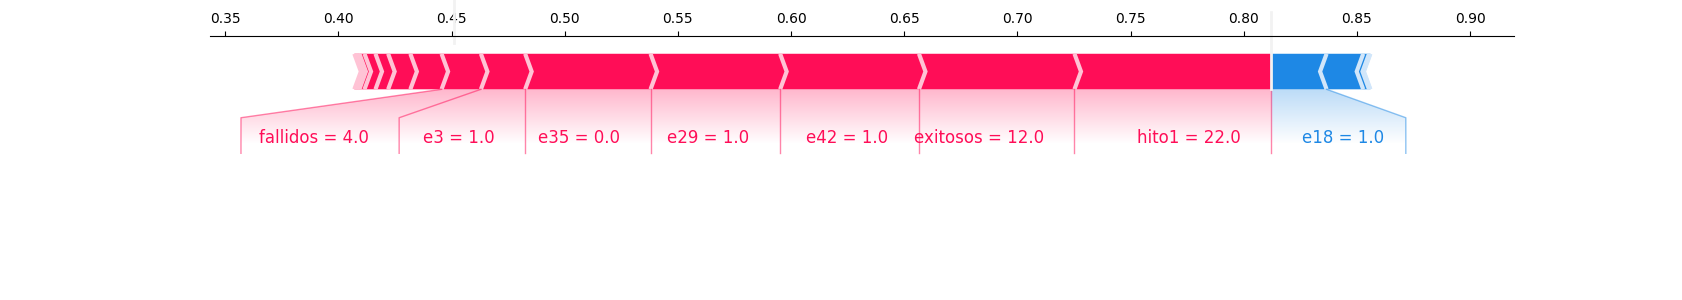
\includegraphics[width=1\textwidth]{img/shap_rf/shapForcePlot.png}
    \caption{Características Variables SHAP (Matplotlib)}
    \label{fig:caract_var_shap_mat}
\end{figure}

Al revisar este gráfico, podemos obtener más detalles sobre las características y su importancia:

\begin{itemize}
    \item La sección \say{higher} muestra los valores positivos que contribuyen a aumentar el valor de predicción. En este caso, \say{hito1} esta mas sercana a la \say{f(x)}, lo que significa que esta característica contribuye positivamente al valor de predicción en conjuntos con las variables \say{exitosos}, \say{e42}, \say{e29}, \say{e35}, \say{e3}, \say{fallidos} para \say{aprobado}.
    \item La sección \say{lower} muestra los valores negativos o fallidos que contribuyen a disminuir el valor de predicción. En este caso, la variable \say{e18}, tiene una contribución negativa al valor de prediccióno que no aporta mucho.
    \item En el gráfico, la marca \say{f(x)} representa el valor de predicción del modelo, que en este caso es 0.81.
    \item En el grafico \say{base value} es el valor promedio de las predicciones del modelo sobre todo el conjunto de datos. Es el punto de partida en el gráfico y representa la predicción que haríamos si no tuviéramos información sobre la instancia en particular.
\end{itemize}

Además de los gráficos anteriores, se presentan los gráficos de dependencia para algunas variables con referencia a \say{aprobado}:

\begin{figure}[H]
    \centering
    \begin{minipage}{0.48\textwidth}
        \begin{lstlisting}[language=Python, caption=Grafico de dependencia hito1, label=lst:grafDepHito1]
# Obtener el índice de la variable "hito1" en tu DataFrame
indice = X.columns.get_loc("hito1")

# Crear el gráfico de dependencia para "hito1"
shap.dependence_plot(indice, shap_values, X_test, feature_names=X.columns, show=False)

# Personalizar la apariencia del gráfico
plt.xlabel("hito1")
plt.ylabel("Valores SHAP")
plt.title("Gráfico de Dependencia")
plt.tight_layout()

# Mostrar el gráfico
plt.show()
        \end{lstlisting}
    \end{minipage}
    \hfill
    \begin{minipage}{0.48\textwidth}
        \begin{lstlisting}[language=Python, caption=Grafico de dependencia e29, label=lst:grafDepE29]
# Obtener el índice de la variable "e29" en tu DataFrame
indice = X.columns.get_loc("e29")

# Crear el gráfico de dependencia para "e29"
shap.dependence_plot(indice, shap_values, X_test, feature_names=X.columns, show=False)

# Personalizar la apariencia del gráfico
plt.xlabel("e29")
plt.ylabel("Valores SHAP")
plt.title("Gráfico de Dependencia")
plt.tight_layout()

# Mostrar el gráfico
plt.show()
        \end{lstlisting}
    \end{minipage}
\end{figure}

\begin{figure}[H]
    \begin{subfigure}{0.48\textwidth}
        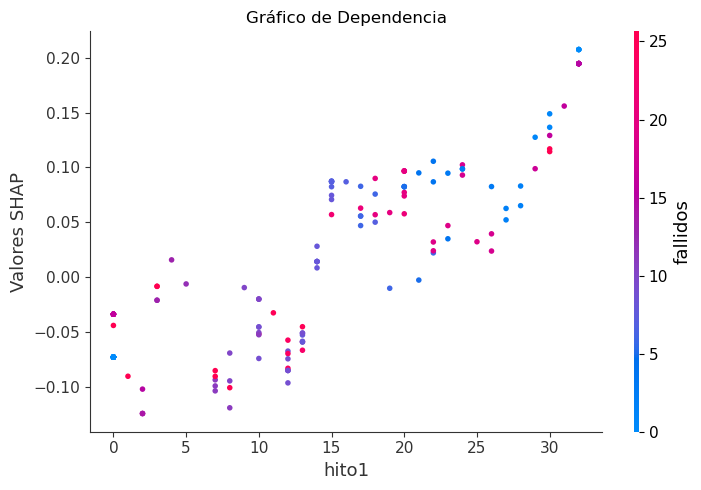
\includegraphics[width=0.9\linewidth, height=6cm]{img/shap_rf/hito1.png}
        \caption{hito1}
        \label{fig:dependencia_hito1}
    \end{subfigure}
    \begin{subfigure}{0.5\textwidth}
        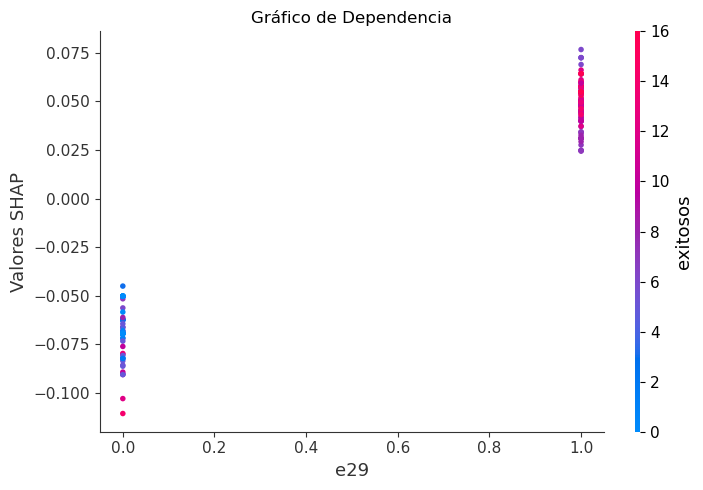
\includegraphics[width=0.9\linewidth, height=6cm]{img/shap_rf/e29.png}
        \caption{e29}
        \label{fig:dependencia_e29}
    \end{subfigure}
    \caption{Variables de dependencias hito1 - e29}
    \label{fig:image1}
\end{figure}

En la Figura \ref{fig:dependencia_hito1} se muestra el gráfico de dependencia para la variable \say{hito1} y refleja \say{fallidos} con su correlación. mientras tanto en la figura \ref{fig:dependencia_e29} se muestra el gráfico de dependencia para la variable \say{e29} con la variable \say{extisoso}.

\begin{figure}[H]
    \centering
    \begin{minipage}{0.48\textwidth}
        \begin{lstlisting}[language=Python, caption=Grafico de dependencia exitosos, label=lst:grafDepExitosos]
# Obtener el índice de la variable "exitosos" en tu DataFrame
indice = X.columns.get_loc("exitosos")

# Crear el gráfico de dependencia para "exitosos"
shap.dependence_plot(indice, shap_values, X_test, feature_names=X.columns, show=False)

# Personalizar la apariencia del gráfico
plt.xlabel("Exitosos")
plt.ylabel("Valores SHAP")
plt.title("Gráfico de Dependencia")
plt.tight_layout()

# Mostrar el gráfico
plt.show()
        \end{lstlisting}
    \end{minipage}
    \hfill
    \begin{minipage}{0.48\textwidth}
        \begin{lstlisting}[language=Python, caption=Grafico de dependencia fallidos, label=lst:grafDepFallidos]
# Obtener el índice de la variable "fallidos" en tu DataFrame
indice = X.columns.get_loc("fallidos")

# Crear el gráfico de dependencia para "fallidos"
shap.dependence_plot(indice, shap_values, X_test, feature_names=X.columns, show=False)

# Personalizar la apariencia del gráfico
plt.xlabel("Fallidos")
plt.ylabel("Valores SHAP")
plt.title("Gráfico de Dependencia")
plt.tight_layout()

# Mostrar el gráfico
plt.show()
        \end{lstlisting}
    \end{minipage}
\end{figure}

\begin{figure}[H]
    \begin{subfigure}{0.48\textwidth}
        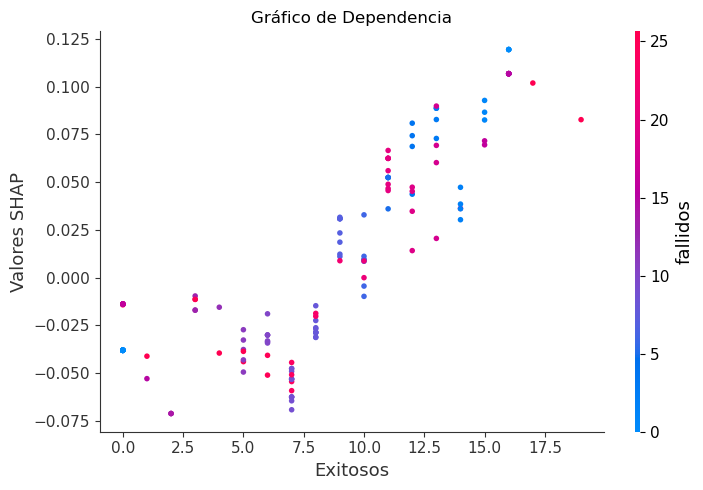
\includegraphics[width=0.9\linewidth, height=6cm]{img/shap_rf/exitosos.png}
        \caption{exitosos}
        \label{fig:dependencia_exitosos}
    \end{subfigure}
    \begin{subfigure}{0.5\textwidth}
        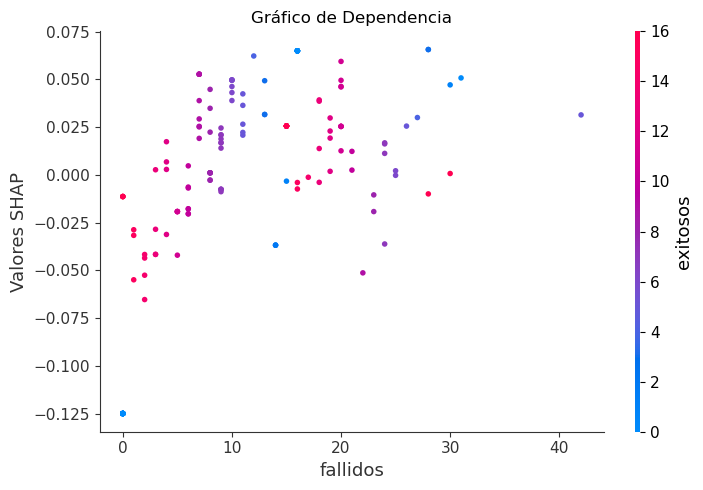
\includegraphics[width=0.9\linewidth, height=6cm]{img/shap_rf/fallidos.png}
        \caption{fallidos}
        \label{fig:dependencia_fallidos}
    \end{subfigure}
    \caption{Variable de dependencias exitosos - fallidos}
    \label{fig:image2}
\end{figure}

En la Figura \ref{fig:dependencia_exitosos} se muestra el gráfico de dependencia para la variable \say{exitosos} con su variable de dependencia \say{fallidos}, mientras tanto en la figura \ref{fig:dependencia_fallidos} se muestra el gráfico de dependencia para la variable \say{fallidos} con su dependencia \say{exitosos}.

\begin{figure}[H]
    \centering
    \begin{minipage}{0.48\textwidth}
        \begin{lstlisting}[language=Python, caption=Grafico de dependencia e42, label=lst:grafDepe42]
# Obtener el índice de la variable "e42" en tu DataFrame
indice = X.columns.get_loc("e42")

# Crear el gráfico de dependencia para "e42"
shap.dependence_plot(indice, shap_values, X_test, feature_names=X.columns, show=False)

# Personalizar la apariencia del gráfico
plt.xlabel("e42")
plt.ylabel("Valores SHAP")
plt.title("Gráfico de Dependencia")
plt.tight_layout()

# Mostrar el gráfico
plt.show()
        \end{lstlisting}
    \end{minipage}
    \hfill
    \begin{minipage}{0.48\textwidth}
        \begin{lstlisting}[language=Python, caption=Grafico de dependencia e3, label=lst:grafDepe3]
# Obtener el índice de la variable "e3" en tu DataFrame
indice = X.columns.get_loc("e3")

# Crear el gráfico de dependencia para "e3"
shap.dependence_plot(indice, shap_values, X_test, feature_names=X.columns, show=False)

# Personalizar la apariencia del gráfico
plt.xlabel("e3")
plt.ylabel("Valores SHAP")
plt.title("Gráfico de Dependencia")
plt.tight_layout()

# Mostrar el gráfico
plt.show()
        \end{lstlisting}
    \end{minipage}
\end{figure}

\begin{figure}[H]
    \begin{subfigure}{0.48\textwidth}
        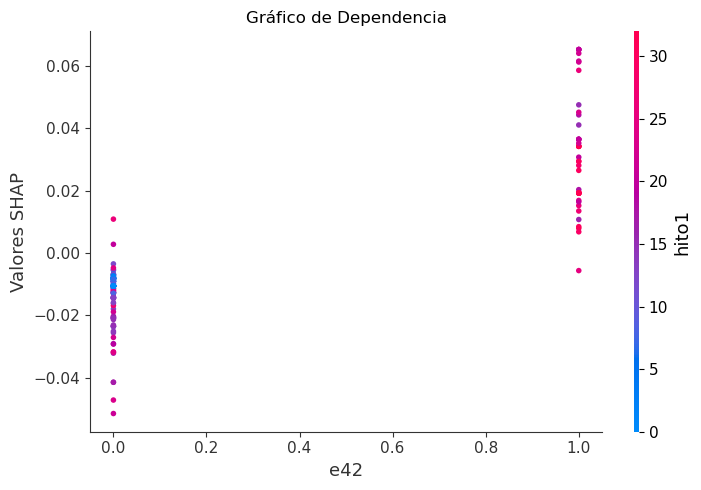
\includegraphics[width=0.9\linewidth, height=6cm]{img/shap_rf/e42.png}
        \caption{e42}
        \label{fig:dependencia_e42}
    \end{subfigure}
    \begin{subfigure}{0.5\textwidth}
        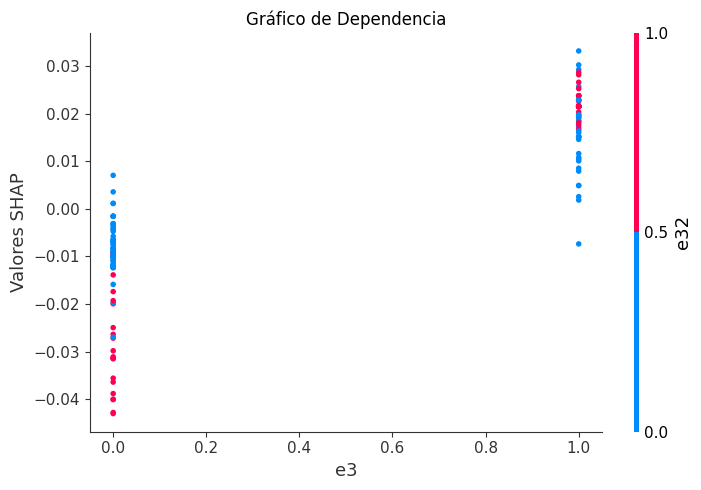
\includegraphics[width=0.9\linewidth, height=6cm]{img/shap_rf/e3.png}
        \caption{e3}
        \label{fig:dependencia_e3}
    \end{subfigure}
    \caption{Variable de dependencias e42 - e3}
    \label{fig:image3}
\end{figure}

En la Figura \ref{fig:dependencia_e42} se muestra el gráfico de dependencia para la variable \say{e42} con su dependencia \say{hito1}, mientras tanto en la figura \ref{fig:dependencia_e3} se muestra el gráfico de dependencia para la variable \say{e3} con la variable \say{e32}.

Estos gráficos de dependencia representan la relación entre los valores de las variables mencionadas y los valores de Shapley en el modelo. Proporcionan una visualización de cómo estas variables influyen en las predicciones del modelo y ayudan a comprender su importancia relativa.


\subsubsection{Reflexiones Finales del Análisis SHAP}

A través del análisis SHAP, hemos obtenido una visión detallada de cómo las distintas características influyen en las predicciones del modelo RandomForestClassifier. Es evidente que ciertas variables tienen un impacto más significativo en la probabilidad de que un estudiante sea clasificado como \textit{\say{aprobado}}.

La variable \say{hito1}, como se observa en la Figura \ref{fig:importancia_relativa_shap}, tiene una contribución positiva considerable, lo que indica que es un factor crucial para determinar la aprobación. Las variables \say{exitosos} y \say{fallidos} también son esenciales, ya que están correlacionadas con la intención de resolver la guía.

Los gráficos de dependencia ofrecen una perspectiva más profunda sobre cómo ciertas variables interactúan entre sí y su relación con la probabilidad de aprobación.

En resumen, el análisis SHAP ha sido instrumental en desentrañar la importancia relativa de las características en nuestro modelo. Estos insights no solo nos permiten entender mejor el comportamiento del modelo, sino que también ofrecen una base sólida para futuras intervenciones educativas, con el objetivo de mejorar las tasas de aprobación y la eficacia de las guías de estudio. Es esencial que, al diseñar estrategias educativas, se consideren estos factores influyentes para garantizar un impacto positivo en el rendimiento de los estudiantes.